\section{Arjun Yuda Firwanda}
\subsection{Teori}
\subsubsection{Apa itu fungsi device manager di windows dan folder /dev di linux}
Fungsi device manager untuk membantu dan mengelola semua hardware yang terpasang dalam suatu windows.

\subsubsection{Jelaskan langkah-langkah instalasi driver dari arduino}
\begin{itemize}
    \item ubungkan sistem minimun Arduino Uno ke komputer dengan kabel USB type B (kabel Printer).
    \item Lalu pada bagian kanan didesktop PC anda, akan muncul popup “Installing device driver software”.
	\item Sistem operasi Windows tidak menyediakan driver untuk Arduino Uno, lalu proses instalasinya harus dilakukan secara manual.
	\item Buka Device Manager, caranya pada bagian Search Program and Files lalu ketikkan “device manager”.
	\item Cari Unknown device pada bagian Other device, terdapat tanda seru yang berwarna kuning, itu disebabkan karena penginstallan tidak berjalan dengan sempurna.
	\item Klik kanan pada “Unknown device”, pilih Update Driver Software.
    \item Pilih Browse my computer for driver software.
	\item Arahkan lokasi folder ke folder arduino-1.0, drivers. Pastikan check-box lalu centang include subfolders. Klik Next untuk melanjutkan instalasi driver.
	\item Kemudian lanjutkan dengan mengklik Install pada tampilan Windows Security.
	\item Jika instalasi driver berhasil maka akan muncul Windows has successfully updated your driver software.
	\item Perhatikan dan ingat nama COM Arduino Uno, karena nama COM ini yang akan digunakan untuk mengupload program nantinya.
\end{itemize}

\subsubsection{Jelaskan bagaimana cara membaca baudrate dan port dari komputer yang sudah terinstall driver}
Untuk baudrate dapat bisa dicek melalui arduino IDE, kemudian untuk mengecek port bisa dilakukan dengan device manager.

\subsubsection{Jelaskan sejarah library pyserial}
Modul ini merangkum akses untuk port serial. Ini menyediakan backends untuk Python yang berjalan di Windows, Linux, BSD (mungkin sistem yang mendukung POSIX), Jython dan IronPython (.NET dan Mono). Modul bernama "serial" secara otomatis memilih backend yang sesuai. Antarmuka berbasis kelas yang sama pada semua platform yang didukung.
Akses ke pengaturan port melalui properti Python. Dukungan untuk berbagai ukuran byte, bit stop, paritas dan kontrol aliran dengan RTS / CTS dan / atau Xon / Xoff. Bekerja dengan atau tanpa menerima batas waktu.
File seperti API dengan "read" dan "write" ("readline" dll. Juga didukung). File-file dalam paket ini adalah 100 persen Python murni. Port diatur untuk transmisi biner. Tidak ada stripping byte NULL, terjemahan CR-LF dll. (Yang berkali-kali diaktifkan untuk POSIX.) Ini membuat modul ini bermanfaat secara universal. Kompatibel dengan pustaka io (Python 2.6+)

\subsubsection{Jelaskan fungsi-fungsi apa saja yang dipakai dari library pyserial}
\begin{itemize}
    \item Serial, fungsi ini untuk membuka port serial
    \item Write(data),  untuk menulis data lewat port serial
    \item Readline, untuk membaca string dari port serial
    \item Read(size), untuk membaca jumlah byte dari port serial
    \item Close, ini untuk menutup port serial 
\end{itemize}

\subsubsection{Jelaskan kenapa butuh perulangan dan tidak butuh perulangan dalam membaca serial}
Perualangan dalam bahasa pemrograman berfungsi untuk menyuruh komputer melakukan sesuatu secara berulang-ulang. Terdapat dua jenis perualangan dalam bahasa pemrograman python diantaranya adalah perulangan dengan for dan while.
Perulangan for atau counted loop (perulangan yang terhitung). Perulangan while atau uncounted loop (perulangan yang tak terhitung). Perbedaannya pada perulangan for biasanya digunakan untuk mengulangi kode yang sudah diketahui banyak perulangannya. Perualangan while untuk perulangan yang memiliki syarat dan tidak tentu berapa banyak perulangannya.
Perualangan digunakan untuk membaca data secara berulang-ulang  dan apabila tidak memakai perulangan, maka data akan terbaca satu per satu.

\subsubsection{Jelaskan bagaimana cara membuat fungsi yang mengunakan pyserial}
\lstinputlisting[firstline=8, lastline=15]{src/5/1174008/teori/T1174008.py}

\subsubsection{Cek Plagiarisme}
\begin{figure}[H]	
    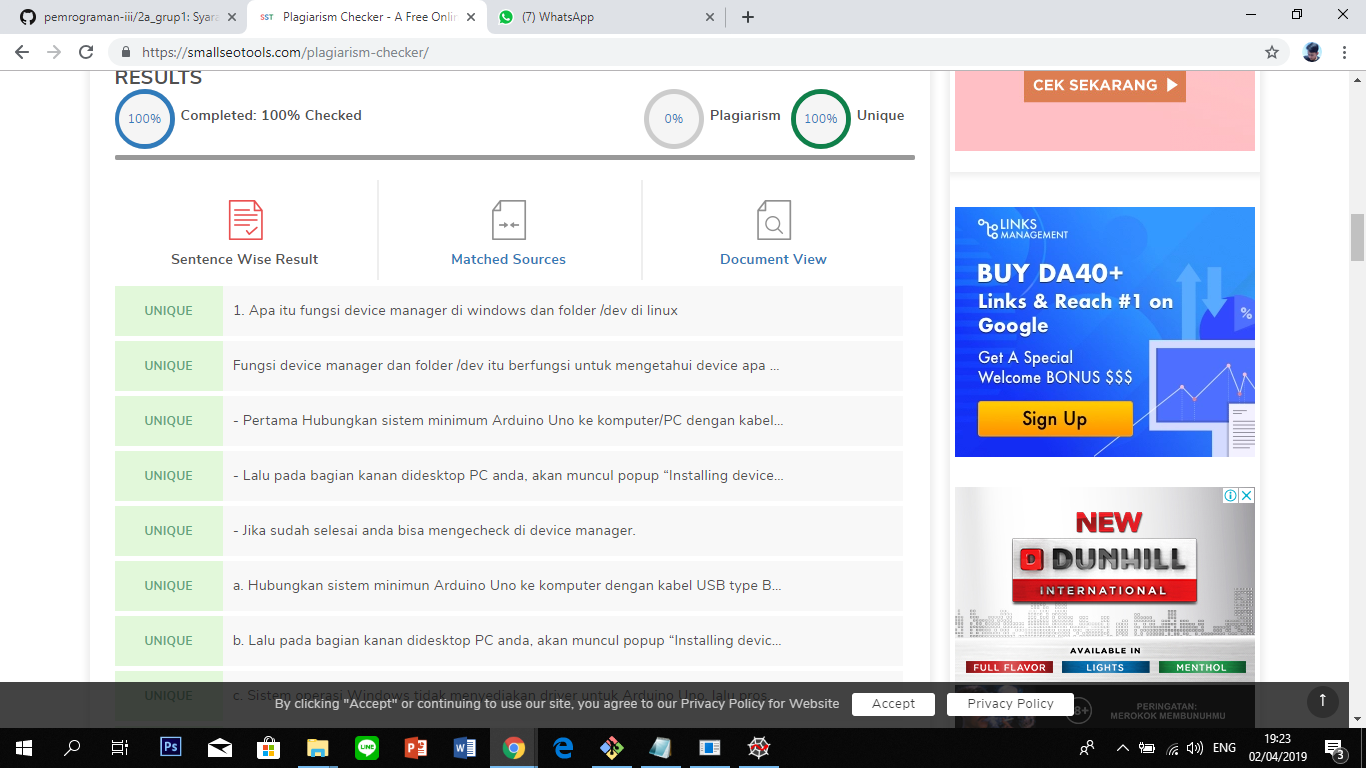
\includegraphics[width=5cm]{figures/5/1174008/teori/ssplagiatchapter5.png}
    \centering
    \caption{Cek Plagiarisme}
\end{figure}

\subsection{Praktek}
\subsubsection{Kerjakan soal berikut ini, ....}
\subsubsection{Penanganan Error}